\documentclass[tikz,border=12pt]{standalone}
\usetikzlibrary{arrows.meta,positioning}
\definecolor{pink}{HTML}{F72585}\definecolor{green}{HTML}{2F9E44}\definecolor{red}{HTML}{E03131}
\definecolor{blue}{HTML}{228BE6}\definecolor{ink}{HTML}{343A40}\definecolor{soft}{HTML}{F1F3F5}
\begin{document}
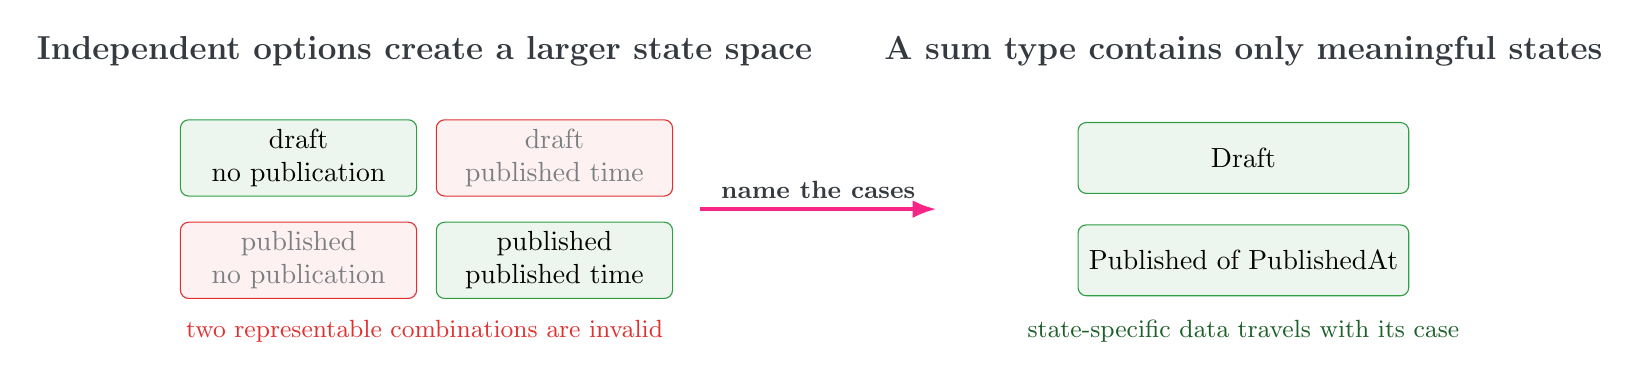
\begin{tikzpicture}[box/.style={rounded corners=3pt,draw=ink!35,fill=soft,minimum width=3cm,minimum height=.9cm,align=center},good/.style={box,draw=green,fill=green!9},bad/.style={box,draw=red,fill=red!7,text=ink!65},arrow/.style={-{Latex[length=3mm]},very thick,pink}]
 \node[font=\bfseries\large,text=ink] at (1.6,3) {Independent options create a larger state space};
 \node[good] at (0,1.65) {draft\\no publication};
 \node[bad] at (3.25,1.65) {draft\\published time};
 \node[bad] at (0,.35) {published\\no publication};
 \node[good] at (3.25,.35) {published\\published time};
 \node[font=\small,text=red] at (1.6,-.55) {two representable combinations are invalid};
 \draw[arrow] (5.1,1)--node[above,font=\small\bfseries,text=ink]{name the cases}(8.1,1);
 \begin{scope}[xshift=10.4cm]
  \node[font=\bfseries\large,text=ink] at (1.6,3) {A sum type contains only meaningful states};
  \node[good,minimum width=4.2cm] at (1.6,1.65) {Draft};
  \node[good,minimum width=4.2cm] at (1.6,.35) {Published of PublishedAt};
  \node[font=\small,text=green!60!black] at (1.6,-.55) {state-specific data travels with its case};
 \end{scope}
\end{tikzpicture}
\end{document}
